\section{Tecnologías implementadas y estado operativo.}
\subsection{Análisis de RAM}
\label{subsec:ramanalisi}
Uno de los puntos más importantes a la hora de implementar un bot con IA para un juego de Atari, es entender cómo está hecho. Utilizaremos el entorno \ac{ale} para extraer características de los juegos, el cual cuenta con una API que nos permite extraer información de los mismos. Para ello, se ha desarrollado un lector de RAM que nos ayuda a visualizar los 128 bytes de memoria de la Atari mientras se ejecuta un juego.

Además, dicho lector implementa colores, lo cual permite que se puedan distinguir las posiciones de RAM que cambian de las que no en un step determinado (paso de ejecución)  como se puede ver en la figura \ref{fig:RAM_Colors}.

\begin{figure}[h]
	\centering
	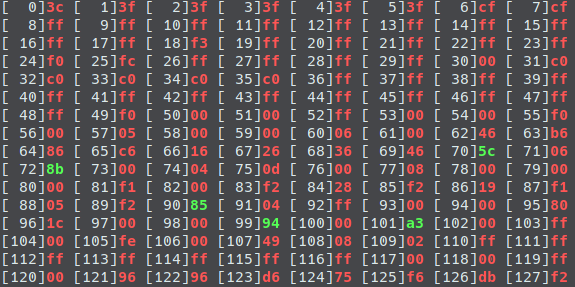
\includegraphics[width=1\textwidth]{Figures/RAMColors}
	\caption{El color verde indica que el valor ha cambiado en este step.}
	\label{fig:RAM_Colors}
\end{figure}

Una de las características de este lector es que acompaña la ejecución con un volcado de analytics para ver las posiciones de RAM que más han cambiado en una ejecución determinada.

Para extraer los datos mas interesantes de un juego en concreto, simplemente hay que observar las posiciones de RAM mas alteradas según nuestro analytics. Una vez hecho esto, se pondrá el juego en cámara lenta gracias a una feature del entorno \ac{ale}, lo cual nos permitirá ver con qué sentido cambian estos valores. Como punto a destacar, no todos los valores que cambian mucho serán relevantes a la hora de sacar datos importantes del juego (un contador podría no ser relevante para un caso específico).

Una vez hecho esto se puede desglosar la RAM de manera bastante precisa, sacando datos como los siguientes.

\begin{figure}[h]
	\centering
	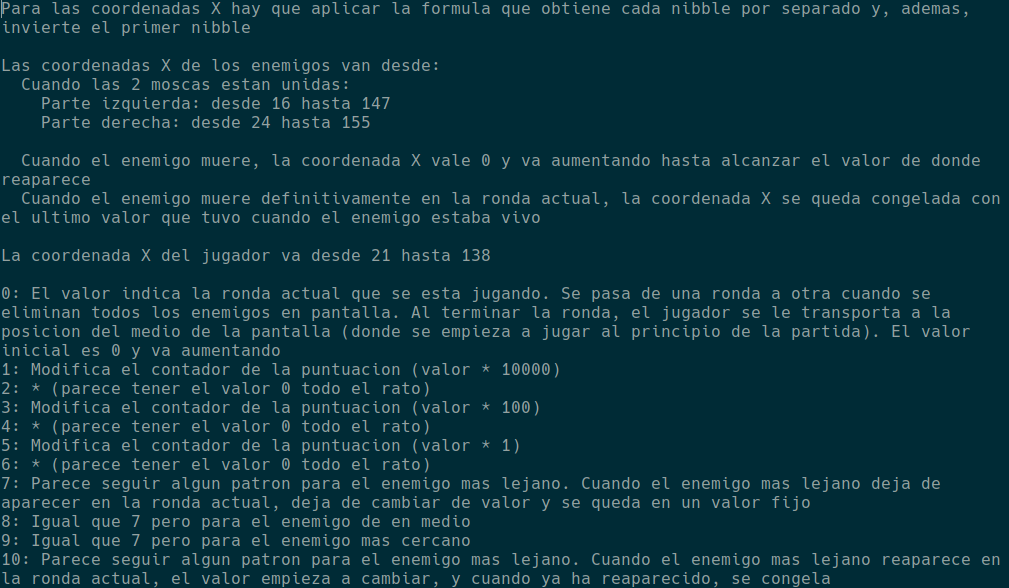
\includegraphics[width=1\textwidth]{Figures/AnalisisRAM}
	\caption{Demon Attack - Análisis de las primeras posiciones de RAM}
	\label{fig:AnalisisRAM}
\end{figure}

Como se puede observar en la figura \ref{fig:AnalisisRAM}, para obtener la información correcta no solo basta con extraer las posiciones relevantes, en algunos casos será necesario procesar esta información. Por ejemplo, en Demon Attack, las coordenadas X de las entidades aparecen ofuscadas de la siguiente manera:

\begin{figure}[h]
	\centering
	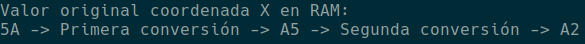
\includegraphics[width=1\textwidth]{Figures/DAttackOpsRequired}
	\caption{Demon Attack - Coordenadas X de las entidades}
	\label{fig:DAttackOpsRequired}
\end{figure}

Como podemos ver en la figura \ref{fig:DAttackOpsRequired}, los nibbles de las coordenadas están invertidos, además, el primer nibble requiere una operación extra, una resta (7 - valor del nibble). 

Una vez tenemos la información recogida y procesada, la podremos utilizar para crear una IA capaz de jugar al juego en concreto. Además de eso, el entorno \ac{ale} cuenta con diversas funcionalidades que nos permiten recoger la información en pantalla en el caso que fuese necesario. 

\subsubsection{Modificando ALE}
\label{subsubsec:ramanalisi:modale}

La primera aproximación que se hizo a la hora de analizar los datos de los diferentes juegos fue básica y útil, pero presentaba varios problemas. El problema más serio que nos encontramos era la cantidad de datos que teníamos ante nuestros ojos, cosa que puede dificultar bastante el encontrar la información importante que necesitamos y, además, que dependemos totalmente de nuestra "intuición" para saber que significa cierta posición de la RAM. Intentando solventar un poco este problema, se nos ocurrió aislar las posiciones que hay en la RAM y, además, poder modificar esos valores aislados para no depender totalmente de nuestra intuición, sino saber más a ciencia cierta, a base de prueba y error, saber qué hace cierta posición de RAM, lo cual nos daría la ventaja de profundizar más en aquellas posiciones de RAM que por alguna razón, en el paso anterior, hemos visto que podían resultar relevantes.

A la hora de intentar poner esta idea en práctica lo primero que intentamos es obtener una referencia de la RAM desde el objeto que hemos ido empleando en todo momento: \textbf{ALEInterface}. Este objeto nos dota del método \textit{getRAM()} que hemos ido utilizando en todo momento para el análisis de los datos (y para posteriormente el tratamiento de los mismos) y que está en el archivo \textit{src/ale\_interface.cpp}. La implementación de dicho método es la siguiente:

\begin{figure}[h]
	\centering
	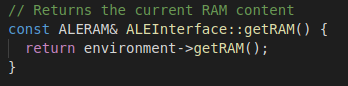
\includegraphics[width=1\textwidth]{Figures/methodGetRAM}
	\caption{Método \textit{getRAM()}}
	\label{fig:methodGetRAM}
\end{figure}

Como observamos, el método \textit{getRAM()} nos devuelve una referencia de un objeto de tipo \textbf{ALERAM}, por lo que vamos a ver que método nos pueden servir para modificar la RAM. Cuando investigamos el archivo \textit{src/environment/ale\_ram.hpp} encontramos la definición del objeto ALERAM y la implementación de sus métodos. Contiene 2 métodos que pueden servirnos para nuestro propósito (modificar la RAM), los cuales se muestran en la siguiente figura.

\begin{figure}[h]
	\centering
	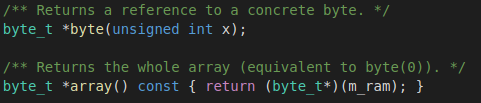
\includegraphics[width=1\textwidth]{Figures/ALEMethodsToGetReferencesToRAM}
	\caption{Métodos de acceso a la RAM de ALEInteface}
	\label{fig:ALEMethodsToGetReferencesToRAM}
\end{figure}

\newpage
Una vez ya encontramos estos métodos, intentamos hacer una pequeña prueba, la cual falla, ya que al intentar hacer uso del método \textit{array()} vemos que modificamos un valor y que, efectivamente, al volver a comprobar el valor, se ha modificado, pero nada sucede en el juego (la prueba la realizamos sobre el videojuego \textit{breakout}, el cual tiene la coordenada X de la barra en la posición 72). Lo que estaba sucediendo, después de indagar un poco por el código de ALE era que el método \textit{getRAM()} de \textit{ale\_interface.cpp} era un método que a su vez llamaba a otro método llamado \textit{getRAM()} pero del objeto \textbf{StellaEnvironment}, objecto que es el encargado de manejar todo el entorno de ALE. Este objeto, de nuevo, devuelve otra vez un objeto de tipo ALERAM por referencia, por lo que de nuevo parece que no hay problema, pero este objeto, \textit{StellaEnvironment}, contiene una copia de la RAM del objeto \textbf{OSystem}, objeto que es el núcleo de la Atari 2600 (del emulador). El problema consiste en que este objeto ALERAM con el que constantemente trabajamos es una copia del que el objeto \textit{OSystem} contiene, es decir, cada vez que llamados al método \textit{getRAM()} desde \textit{ale\_interface.hpp}, se hace otra llamada al método \textit{getRAM()} de \textit{src/environment/stella\_environment.cpp} y este devuelve su copia interna, no la del núcleo de la consola. Cada vez que el objeto \textit{StellaEnvironment} actualiza su copia hace uso del método \textit{processRAM()}.

\begin{figure}[h]
	\centering
	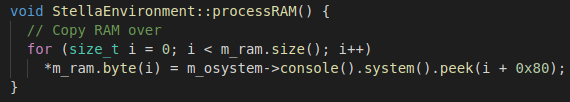
\includegraphics[width=1\textwidth]{Figures/StellaEnviromentProcessRAMMethod}
	\caption{Método \textit{processRAM()} de StellaEnviroment}
	\label{fig:StellaEnviromentProcessRAMMethod}
\end{figure}

Una vez llegado a este punto, lo que se puede hacer si se quiere modificar la RAM que contiene el objeto \textit{OSystem} es implementar un método que lo que haga es actualizar la RAM del objeto \textit{OSystem} del mismo método que que podemos observar que se puede obtener una copia de la RAM con su método \textit{console().system().peek()}, pero tenemos que comprobar si existe el método que nosotros necesitamos, y es que en vez de \textit{peek()} necesitamos un método que nos permita actualizar. De nuevo, buscando en el código, encontramos el archivo \textit{src/emucore/OSystem.hxx}, el cual nos lleva al archivo \textit{src/emucore/Console.hxx}, el cual nos lleva, finalmente, al archivo \textit{src/emucore/System.hxx}. En este último encontramos el método \textit{poke(uInt16, uInt8)}, el cual nos indica a través de su descripción que modifica un valor de la RAM de la consola Atari 2600. Parece ser que ya lo tenemos todo, pero nos queda un último problema, y es que este método no es accesible desde el objeto \textit{StellaEnvironment}, ya que su referencia del objeto \textit{OSystem}, a diferencia del objeto \textit{ALEInterface}, está en su parte privada y no nos da ningún método público para obtener una copia de la referencia. El último paso que nos queda para solucionar este último problema es modificar el código y añadir un método que nos permita actualizar la RAM de la Atari 2600 a partir de la copia que tiene internamente el objeto \textit{StellaEnvironment}, ya que esta última sí que podemos modificarla.

\begin{figure}[h]
	\centering
	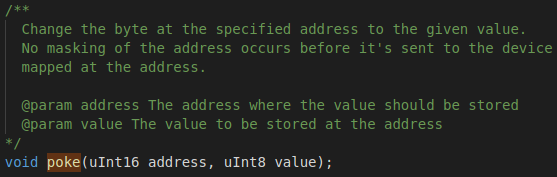
\includegraphics[width=1\textwidth]{Figures/pokeMethod}
	\caption{Método \textit{poke(uInt16, uInt8)}}
	\label{fig:pokeMethod}
\end{figure}

El método que hemos implementado es muy sencillo. Es igual que el método \textit{processRAM()} pero utilizando el método \textit{poke()} en vez de \textit{peek()}. Una vez ya implementado el método, simplemente implementamos otro método en el objeto \textit{ALEInterface} que simplemente haga una llamada a este método que está en el objeto \textit{StellaEnvironment} y ya habremos actualizado la RAM de la Atari 2600. Por último solo quedaría recompilar ALE. Este proceso que hemos realizado a sido con el único objetivo de comprender mejor el significado de las posiciones de RAM de los diferentes juegos a analizar durante este trabajo. Se adjuntarán para cada juego un archivo denominado \textbf{RAM.txt} en el cual hemos analizado cada posición de RAM de manera aislada.

\begin{figure}[h]
	\centering
	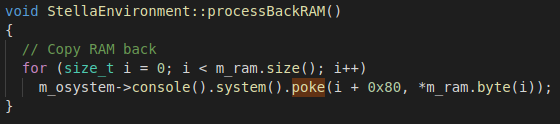
\includegraphics[width=1\textwidth]{Figures/processBackRAM}
	\caption{Método que actualiza la RAM de la Atari 2600}
	\label{fig:processBackRAM}
\end{figure}

\newpage
\subsection{Bots básicos}
\label{subsec:botsbasicos}
Se han desarrollado bots semi-deterministas empleando técnicas básicas de inteligencia artificial para poder extraer datos de gameplay. Los primeros volcados de datos se hicieron con operarios humanos jugando a los juegos, pero al ver que nuestras scores eran mas bien bajas, se optó por implementar IA básica para cada uno de los juegos. 

Estas implementaciones básicas mejoraron mucho las scores obtenidas, por lo que los datos extraídos de los bots eran mas afines a obtener mayores puntuaciones que los nuestros.

Además, sobre esta IA básica, se pueden hacer iteraciones de mejora, teniendo en cuenta más datos o mas información en pantalla, como se ha comentado anteriormente en la subsección \ref{subsec:ramanalisi}.

Este scripting básico ayudará mas adelante a la implementación utilizando machine learning, ya que los datos extraídos y procesados para la implementación básica serán utilizados por el algoritmo de machine learning.

A continuación, describiremos cada uno de los bots básicos y su funcionamiento al igual que algunos detalles de implementación.

\subsubsection{Plantilla común}
\label{subsec:botsbasicos:plantcomun}
Todos los bots comparten una serie de utils que analizaremos a continuación.

\begin{figure}[h]
	\centering
	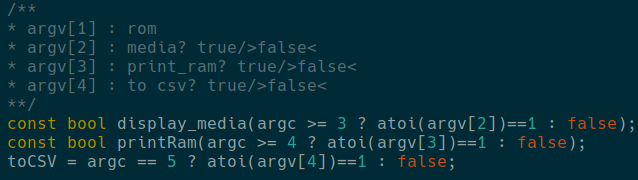
\includegraphics[width=1\textwidth]{Figures/ALEMediaSettings}
	\caption{Opciones de ejecución}
	\label{fig:ALEMediaSettings}
\end{figure}

argv 1 es la ROM que utilizará nuestro ejecutable, argv 2 se corresponde con el contenido multimedia (video y audio), argv 3 escribirá la RAM en consola y argv 4 exportará los datos de gameplay a un archivo \ac{csv} si así se requiere. Se han parametrizado estas opciones porque las ejecuciones son mucho mas lentas conforme mas información requiramos, esto se nota sobre todo a la hora de desactivar el contenido multimedia.

\begin{figure}[h]
	\centering
	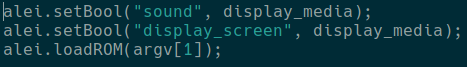
\includegraphics[width=0.7\textwidth]{Figures/ALEromANDmedia}
	\caption{La ROM y el contenido multimedia corren a cargo de \ac{ale}.}
	\label{fig:ALEromANDmedia}
\end{figure}

\newpage
Algunas de estas opciones corren a cargo del entorno (Figura 	\ref{fig:ALEromANDmedia}), mientras que las otras han sido implementadas por nosotros.

Otra de las partes comunes a todos los bots es el bucle principal de ejecución que podemos ver a continuación en la figura \ref{fig:ALEMainExecLoop}. Este bucle está situado en \textbf{main()} y es el encargado de analizar y ejecutar las acciones requeridas en cada step del juego en activo.

\begin{figure}[h]
	\centering
	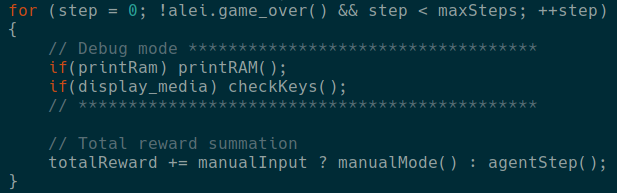
\includegraphics[width=1\textwidth]{Figures/ALEMainExecLoop}
	\caption{Bucle principal de ejecución.}
	\label{fig:ALEMainExecLoop}
\end{figure}

En este bucle observamos nuestra opción \textbf{printRam} que llama al método encargado de imprimir la RAM, el cual convierte a hexadecimal cada uno de los valores de RAM obtenidos mediante el método \textbf{getRAM().get(i)} del entorno \ac{ale}, además hace un seguimiento de los valores de RAM del step anterior para comprobar si dichos valores han cambiado como hemos visto anteriormente en la figura \ref{fig:RAM_Colors}.

Otra opción que encontramos en el bucle principal de ejecución es \textbf{display\_media}, pero en este caso es usado para llamar al método \textbf{checkKeys()}, esto se hace porque no tiene sentido trackear el input si no existe contenido de video. Este método de input es propio, ya que el método de input de ALE "pausa" el agente, lo cual no nos interesa para extraer datos. \textbf{checkKeys()} simplemente activa o desactiva el modo manual propio con la tecla "E", reflejado en la variable \textbf{manualInput}.

La variable \textbf{manualInput} decidirá que función se llama para calcular \textbf{totalReward}. \textbf{manualMode()} mapea el teclado a diferentes acciones del juego, mientras que \textbf{agentStep()} es el bot autónomo específico a cada juego.

Otra de las partes comunes a todos los agentes es la parte de volcado de datos, para ello se han implementado dos funciones de escritura que imprimen strings o dobles en el archivo \ac{csv} anteriormente comentado, como bien podemos ver en la figura .

\begin{figure}[h]
	\centering
	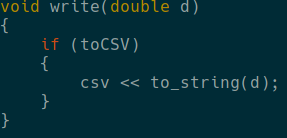
\includegraphics[width=0.4\textwidth]{Figures/aledumpcsv}
	\caption{Una de las funciones de escritura en CSV.}
	\label{fig:aledumpcsv}
\end{figure}


\subsubsection{Breakout}
\label{subsec:botsbasicos:breakout}
El Breakout es el juego mas simple de todos los que analizaremos en esta parte de la sección, pues el número de inputs que tiene es mas bien pequeño. En el Breakout contamos con un total de 5 vidas para pasarnos los 2 niveles de los que dispone. El Breakout fue el primer juego en el que vimos la necesidad de automatizar al jugador, ya que la velocidad de la pelota va incrementando en función a los ladrillos restantes que quedan, lo cual provocaba que perdiésemos siempre en este punto.

\begin{figure}[h]
	\centering
	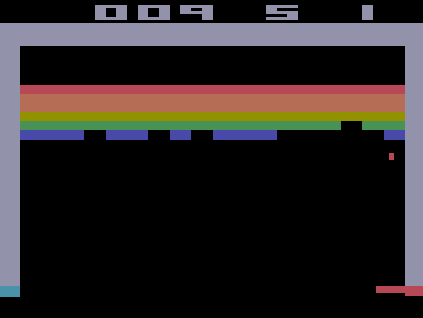
\includegraphics[width=0.7\textwidth]{Figures/breakoutgame}
	\caption{Juego Breakout.}
	\label{fig:breakoutgame}
\end{figure}

Simplemente proporcionando la posición X de la pelota y de la pala al bot y moviendo la pala hacia la pelota, el agente ya jugaba bastante bien. Una mejora que se hizo al algoritmo es hacer un control del tamaño de la pala, al igual que en vez de tener en cuenta solo la posición actual de la pelota, añadir a los datos la posición anterior. Con todas estas mejoras la puntuación se maximizó hasta el punto en el cual el agente fue capaz de pasarse el juego completo. A continuación se muestra en el algoritmo \ref{alg:breakoutimpl}
el pseudocódigo de la IA del Breakout.

\vspace{4mm}
\begin{algorithm}[H]
	\If{lives() != lastLives}{
		$--$lastLives\;
		act(FIRE)\;
	}
	
	wide := getRAM.get(108)\;
	playerX := getPlayerX()\;
	ballX := getBallX()\;
	
	\If{$BallX\_LastTick < ballX$}{
		ballX $+= ((rand() \% 2) + 2);$
	}
	\If{$BallX\_LastTick > ballX$}{
		ballX $-= ((rand() \% 2) + 2);$
	}

	ballX\_LastTick := getBallX()\;
	
	\eIf{$ballX < playerX + wide$}{
		reward $+= act(LEFT);$
	}{
		\If{$(ballX > playerX + wide) \&\& (playerX + wide < 188)$}{
			reward $+= act(RIGHT);$
		}
	}
	\caption{Breakout agent}
	\label{alg:breakoutimpl}
\end{algorithm}

Si analizamos el pseudocódigo anterior, podemos ver cuatro partes. En la primera parte, constituida por el primer if, vemos como el agente presiona la tecla \textbf{FIRE} cuando pierde una vida, esto se debe a que en Breakout cuando pierdes una vida tienes que sacar la pelota pulsando esa tecla. 

En la segunda parte recogemos los datos principales, en este caso \textbf{wide}, que corresponde al ancho de la pala, además de \textbf{playerX} y \textbf{ballX}. 

La tercera parte calcula la dirección de la bola, esto se saca comprobando la posición anterior de la bola con la actual en el eje X, una vez sabemos la dirección aplicamos una suma con un poco de aleatoriedad (para evitar ejecuciones deterministas) en la dirección recogida. Una vez hecho eso nos guardamos la posición de la pelota para la siguiente iteración.

En la cuarta parte aplicaremos el input en función a la posición del jugador respecto a la pelota, teniendo en cuenta el ancho de la pala recogido anteriormente.

\subsubsection{Boxing}
\label{subsec:botsbasicos:boxing}
Boxing es un juego en el cual controlamos a un boxeador y tenemos que asestar mas golpes que el rival para ganar la ronda. En este juego tuvimos los mismos problemas que con el Breakout, por lo que decidimos implementar otro bot, el cual jugaba mejor que nosotros, lo que se resumía en todo ventajas.

\begin{figure}[h]
	\centering
	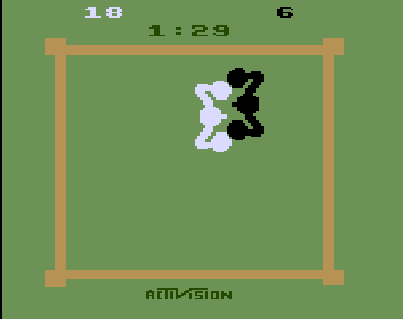
\includegraphics[width=0.7\textwidth]{Figures/boxing}
	\caption{Juego Boxing.}
	\label{fig:boxing}
\end{figure}

En este agente hemos tomado una estrategia agresiva, si el rival lanza un puñetazo, lo intentaremos bloquear con nuestros propios puños poniendo a nuestro boxeador exactamente en la misma posición "Y" que el boxeador contrario (una de las features de Boxing es que la colisión de los puños bloquea los golpes). Además, nuestro boxeador nunca se moverá hacia la izquierda, solo se mueve hacia la derecha en posición de ataque intentando posicionarse en la "Y" del rival, como hemos comentado antes. A su vez, basándonos en ciertas tolerancias, se atacará siempre que sea posible. Esta estrategia agresiva funciona una gran mayoría de las veces, además para evitar el determinismo se ha implementado una pequeña aleatoriedad cada vez que recogemos las posiciones del jugador 1 y del jugador 2 de RAM, como bien se puede ver en el ejemplo de la figura \ref{fig:boxingAleatoriedad}.

\begin{figure}[h]
	\centering
	\includegraphics[width=0.7\textwidth]{Figures/boxingAleatoriedad}
	\caption{Uso de \textbf{rand()} para evitar el determinismo.}
	\label{fig:boxingAleatoriedad}
\end{figure}

A continuación se muestra en el algoritmo \ref{alg:boxingimpl}, la IA implementada. Un detalle a comentar antes de entrar a analizar el algoritmo es que \textbf{player\_pos} es un tipo de dato struct.

%\vspace{2mm}
\begin{algorithm}[H]
	player\_pos p1(getP1\_X(), getP1\_Y())\;
	player\_pos p2(getP2\_X(), getP2\_Y())\;
	absp1p2X := abs(p1.x - p2.x)\;
	absp1p2Y := abs(p1.y - p2.y)\;
	
	\eIf{$absp1p2Y > 3$ \&\& $absp1p2Y < 20$}{
		reward $+= act(FIRE);$
	}{
		\eIf{$absp1p2X > 25$ \&\& $absp1p2X < 40$}{
			reward $+= act(RIGHT);$
		}{
			reward += $(p1.y > p2.y)$ ? act(UP) : act(DOWN)\;
		}
	}
	\caption{Boxing agent}
	\label{alg:boxingimpl}
\end{algorithm}

En la primera parte de recogida de datos, encapsulamos en un struct la posición del jugador uno y la del jugador dos, extrayéndolos de RAM. Como ya hemos comentado anteriormente, estas posiciones implementan una aleatoriedad mínima para evitar ejecuciones deterministas. Además, en la misma sección, calcularemos la distancia entre ambos jugadores en "X" y en "Y", representadas en \textbf{absp1p2X} y \textbf{absp1p2Y} respectivamente, para luego utilizarlas mas adelante.

Una vez tenemos todos los datos procesados, observaremos si nos encontramos en un rango de tolerancia "Y" válido para atacar, si lo estamos, atacaremos (como punto a destacar, este rango es bastante amplio para enfatizar esta estrategia ofensiva). Si no podemos atacar, nos moveremos hacia la derecha  con ciertas tolerancias, o nos situamos en la "Y" del enemigo.


\subsubsection{Demon Attack}
\label{subsec:botsbasicos:da}
El Demon Attack es un juego en el cual controlamos a una nave con un patrón de movimiento similar al Space Invaders. Tendremos que disparar a las naves rivales para pasar de fase además de evitar todo contacto enemigo. El jugador cuenta con una serie de vidas para pasarse los niveles, si estas vidas se acaban el juego termina. De nuevo, vimos la necesidad de crear un bot debido a las bajas puntuaciones obtenidas.

\begin{figure}[h]
	\centering
	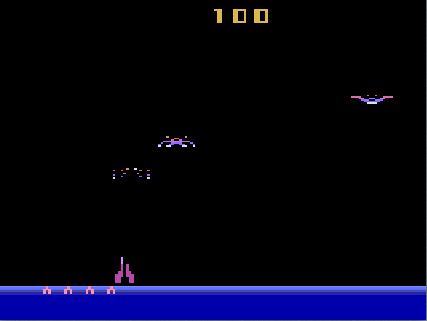
\includegraphics[width=0.9\textwidth]{Figures/demonAttackOne}
	\caption{Juego Demon Attack.}
	\label{fig:demonattackone}
\end{figure}

El Demon Attack es, sin duda, uno de los juegos mas complejos con los que hemos tenido que lidiar, debido a la cantidad de entidades en pantalla, desde disparos hasta múltiples enemigos. La estrategia de IA seguida en el Demon Attack es compleja debido al factor de la gran cantidad de entidades, pues no solo leemos valores en RAM, sino que aprovechamos la característica de \ac{ale} que nos permite leer los píxeles de la pantalla.

Al analizar la RAM, observamos que habían demasiadas características a tener en cuenta, a pesar de tener un análisis detallado de la misma. Hay posiciones de RAM que representan varias cosas en diferentes situaciones, un ejemplo es el valor representado por \textit{RAM[20]}: 

\newpage
\textit{"20: Coordenada "X" de las balas del enemigo. También es la coordenada "X" de la mosca que se acerca para intentar matar al jugador 1 (se utiliza como una bala). Va desde 29 hasta 147 (incluso cuando dispara la mosca). El valor es todo el rato el mismo hasta que el enemigo dispara y actualiza la coordenada. Si hay mas de 2 cambios consecutivos en 2 frames significa que no es una bala y que es la mosca que sigue al jugador"}.

Es por ello por lo que se dedujo que para implementar un bot básico (sin machine learning), era más fácil hacer un análisis de lo que estuviera pasando en la pantalla en un instante determinado, sin dejar de lado la RAM. Para esto, se diseñó un método de visión en el cual la nave es capaz de ver y filtrar enemigos en un área de visión y actuar concorde la situación dependiendo de unas reglas determinadas. En la figura \ref{fig:demonAttackVision} se puede observar el área de visión de la nave.

\begin{figure}[h]
	\centering
	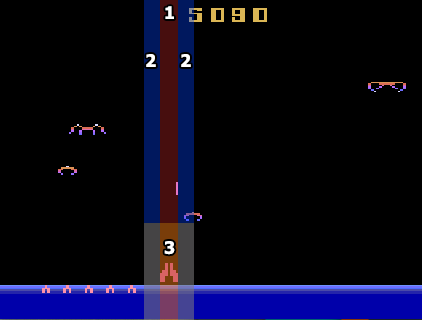
\includegraphics[width=1\textwidth]{Figures/demonAttackVision}
	\caption{Vision de la nave.}
	\label{fig:demonAttackVision}
\end{figure}

La visión de la nave se divide principalmente en 3 partes. En la figura vemos una línea roja representada con el número 1, esta línea roja representa la visión de la nave en función a la anchura de la misma. El número 2 es un area parametrizable que permite ampliar esta visión de forma simétrica por los dos lados de la nave. Tanto el rectángulo rojo como el azul se extienden por casi toda la "Y" de la pantalla y lo único que filtran son los disparos enemigos, como los disparos enemigos tienen el mismo color es muy simple filtrarlos. Por lo tanto 1 y 2 se encargan de detectar disparos enemigos, una vez detectados se actuará en consecuencia.

El número 3 es un área reducida dentro del área completa que se encarga de detectar todas las posibles amenazas, no solo disparos, que estén cerca de la nave. Es decir, el objetivo de la visión es la detección de entidades peligrosas en un área de riesgo para posteriormente evitarlas.

El seguimiento de enemigos para atacarles y matarlos corre a cargo de la RAM, aunque no es del todo exacto debido al problema comentado anteriormente de posiciones de RAM no especificas a una única funcionalidad.

Para analizar la parte práctica de éste algoritmo es necesario separarlo en distintas partes, detección, esquiva y seguimiento.

La parte de detección funciona recogiendo la pantalla entera en grayscale, esto lo hacemos gracias a una funcionalidad de \ac{ale}, una vez tenemos la pantalla guardada, podemos ver cual es el valor de cada píxel. Gracias a esto, podemos determinar el color de los disparos y de las naves enemigas, los que guardaremos en las siguientes variables para después su posterior filtrado:

\begin{figure}[h]
	\centering
	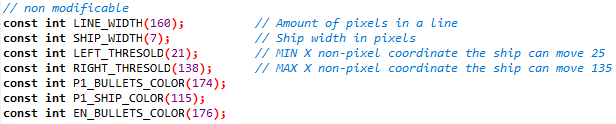
\includegraphics[width=1\textwidth]{Figures/demonAttackStaticOne}
	\caption{Constantes fijas relativas a la visión de la nave.}
	\label{fig:demonAttackStaticOne}
\end{figure}

En la figura \ref{fig:demonAttackStaticOne} podemos observar diversas constantes, entre ellas el color de las balas del jugador 1, \textbf{P1\_BULLETS\_COLOR}, el color de la nave del jugador 1, \textbf{P1\_SHIP\_COLOR} y el color de las balas enemigas, \textbf{EN\_BULLETS\_COLOR}. Gracias a estar en grayscale, con tener un solo valor es suficiente. Además podemos observar otras constantes como \textbf{LINE\_WIDTH}, que representa el ancho en píxeles de la resolución de la Atari, \textbf{SHIP\_WIDTH}, el ancho en píxeles de la nave y \textbf{LEFT / RIGHT\_THRESOLD}, que es la coordenada "X" mínima y máxima en la que se puede mover la nave aliada.

\newpage
Además de estas constantes, Demon Attack cuenta con cuatro constantes adicionales que nos permiten parametrizar algunas características de nuestro algoritmo, como se puede ver en la figura \ref{fig:demonAttackChangableOne} .

\begin{figure}[h]
	\centering
	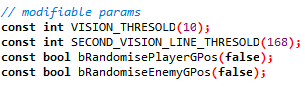
\includegraphics[width=0.7\textwidth]{Figures/demonAttackChangableOne}
	\caption{Constantes modificables (no runtime).}
	\label{fig:demonAttackChangableOne}
\end{figure}

La primera variable de la figura representa el área extra de visión 2 definida en la imagen \ref{fig:demonAttackVision}, la segunda variable define en que línea empieza el área de visión 3. Las dos variables restantes es aleatoriedad opcional a la hora de recoger las posiciones, como se ha hecho antes en el \textit{Boxing}. En este caso, debido a la gran cantidad de entidades en pantalla se ha optado por deshabilitar la aleatoriedad y hacer las batallas mas deterministas.

Otro dato a remarcar antes de empezar con el algoritmo es el Enum utilizado para las colisiones:

\vspace{4mm}
\begin{algorithm}[H]
	enum BlockingHit \{
		$EMoveRight,$
		$EMoveLeft,$
		$ENotBlocking$
	\};
	\caption{Enum empleado para las colisiones.}
	\label{alg:enumcoli}
\end{algorithm}

\vspace{4mm}
Para entender el Enum del algoritmo \ref{alg:enumcoli} tenemos primero que comprender las respuestas que puede dar una colisión y como se operan. 

\begin{itemize}
	\item \textbf{EMoveRight}: La amenaza se ha detectado en la parte izquierda de nuestra área de visión, para contrarrestarla nos moveremos a la derecha si podemos.
	\item \textbf{EMoveLeft}: La amenaza se ha detectado en la parte derecha de nuestra área de visión, para contrarrestarla nos moveremos a la izquierda si podemos.
	\item \textbf{ENotBlocking}: No se ha detectado amenaza ninguna.
\end{itemize}

\newpage
Una vez que ya sabemos qué indicadores utilizaremos para las colisiones, podemos proceder a despiezar el algoritmo.

\begin{figure}[h]
	\centering
	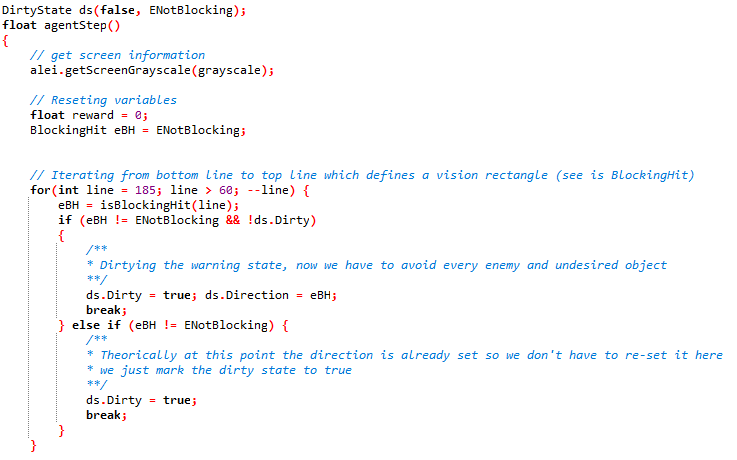
\includegraphics[width=1\textwidth]{Figures/demonattackp1algo}
	\caption{Primera parte del algoritmo de IA para el Demon Attack.}
	\label{fig:demonattackp1algo}
\end{figure}

En esta primera parte recogemos los píxeles de la pantalla con la funcionalidad de \ac{ale} \textbf{getScreenGrayscale}, para luego emplearlos dentro del bucle en la función \textbf{isBlockingHit(int)}, que analizaremos mas adelante. Este bucle se encarga de recorrer 125 filas de la pantalla. En función a la respuesta de \textbf{isBlockingHit(int)}, marcará una variable a true, la cual representa que ha habido una colisión, además dentro de este struct \textbf{DirtyState}, disponemos de otra variable de tipo EBlockingHit para marcar también la dirección contraria a la colisión dada por isBlockingHit. Se ha decidido este thresold ya que el resto de líneas de pantalla contienen información no relevante para el problema.

Para resumir esta parte del código, marcamos el estado a Dirty y recogemos la dirección conveniente, siempre que isBlockingHit haya detectado una colisión. Hasta que no salimos del estado Dirty, no podremos recoger nuevas direcciones, pero de ello se encargará otra parte del código. Es decir, teóricamente se ha implementado una mini máquina de estados finita (FSM), ya que la nave posee dos estados principales (dirty y no dirty) y la forma de transicionar entre ellos es mediante el código de colisiones.

\newpage
\begin{figure}[h]
	\centering
	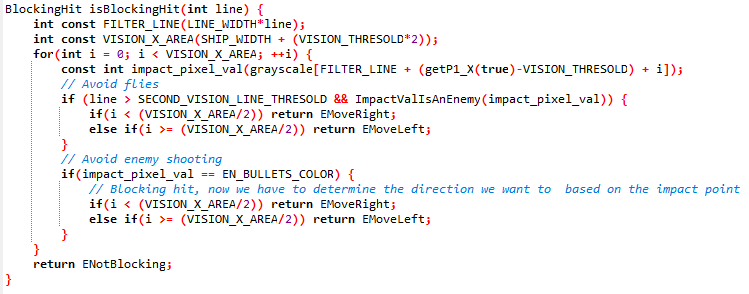
\includegraphics[width=1\textwidth]{Figures/daisblocking}
	\caption{Función isBlockingHit.}
	\label{fig:daisblocking}
\end{figure}

La función isBlockingHit tiene que ser capaz de recorrer el array obtenido por \textbf{getScreenGrayscale} de manera eficiente. Para ello lo primero que hace es resolver la posición del array que ocupa el primer píxel de la línea a analizar, esto es fácil, pues simplemente multiplicando el ancho de la línea con el número de línea ya tenemos este número (asumiendo que las líneas empiezan en 0).

La siguiente tarea es resolucionar el thresold, el cual consiste en el área que ocupa la nave, en este caso 7, mas el thresold determinado, que en nuestro caso corresponde al número de píxeles extras que tendremos en cuenta en cada lado, por ejemplo, si el thresold es 2, el área total será 7+2+2 = 11.

La iteración que haremos en el bucle irá desde 0 hasta el área total que ocupa la visión de la nave, esto es, como ya hemos dicho anteriormente, el área de la nave mas el thresold. Esto hace que solo iteremos los píxeles necesarios para nuestra situación.

La primera línea que encontramos en el bucle puede parecer confusa, pero tiene su explicación:

\vspace{2mm}
\begin{algorithm}[H]
    const int impact\_pixel\_val(grayscale[FILTER\_LINE + (getP1\_X(true)-VISION\_THRESOLD) + i]);
	\caption{Calculo del valor del píxel en un punto determinado de nuestra area de visión.}
	\label{alg:weirdlineda}
\end{algorithm}
\vspace{2mm}

Necesitamos el valor del píxel en un punto determinado de nuestra área de visión. Para ello, necesitamos pedirle al array grayscale esta información, pero antes necesitamos calcular qué posición del array es la correcta. Al haber pre-calculado la posición del array del primer píxel de la línea lo tenemos mucho mas fácil, pues tenemos por donde empezar. A ese número le tenemos que sumar la posición del jugador uno, representado en \textbf{getP1\_X(true)}, al cual le pasamos el parámetro true para que nos devuelva la posición en píxeles, la cual es más precisa para este problema. Una vez tenemos la posición del jugador solo nos queda sumarle i para abordar todo el área de visión. Pero como bien podemos observar en el algoritmo \ref{alg:weirdlineda}, estamos restando a la posición del jugador el \textbf{VISION\_THRESOLD}, esto se hace porque sino estaríamos solo teniendo en cuenta el área extra por la derecha, ya que la colisión estaría desplazada a la izquierda como muestra la figura 	\ref{fig:colisioncalculadaerroneamenteda}, por ello es necesario restar \textbf{VISION\_THRESOLD}.,

\begin{figure}[h]
	\centering
	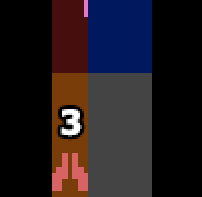
\includegraphics[width=0.3\textwidth]{Figures/colisioncalculadaerroneamenteda}
	\caption{Area de sin restar VISION\_THRESOLD al jugador.}
	\label{fig:colisioncalculadaerroneamenteda}
\end{figure}

Una vez hemos resolucionado el valor del píxel, podemos hacer el filtrado del mismo, el cual se realizará en el cuerpo del bucle.

\begin{figure}[h]
	\centering
	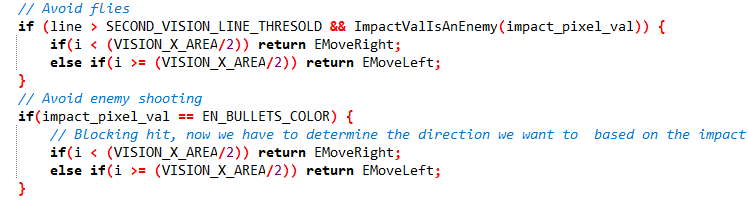
\includegraphics[width=1\textwidth]{Figures/cuerpobucleisblockingda}
	\caption{Resolución de la colisión}
	\label{fig:cuerpobucleisblockingda}
\end{figure}

Como bien observamos en la figura 	\ref{fig:cuerpobucleisblockingda}, haremos una primera distinción para las moscas y enemigos mas cercanos a nuestra segunda área de visión seguido de la visión normal. Priorizamos el segundo área de visión porque está mas cerca del jugador, lo cual se traduce en más peligro a perder una vida. En el primer if, miramos si nos encontramos en el área de riesgo y filtramos por color principalmente si lo que hay en ese píxel es un enemigo. Si es así, es que ha habido una colisión. Si la i en la cual nos encontramos es menor (o está a la izquierda) de la mitad del área de visión, nos moveremos a la derecha (camino más corto para evitar la colisión). Haremos lo mismo para el otro ladro. El segundo if es exactamente lo mismo solo que nos centramos únicamente en las balas enemigas.

Finalmente, si no se ha encontrado colisión ninguna, como hemos visto en la figura \ref{fig:daisblocking}, devolveremos \textit{ENotBlocking}.

\begin{figure}[h]
	\centering
	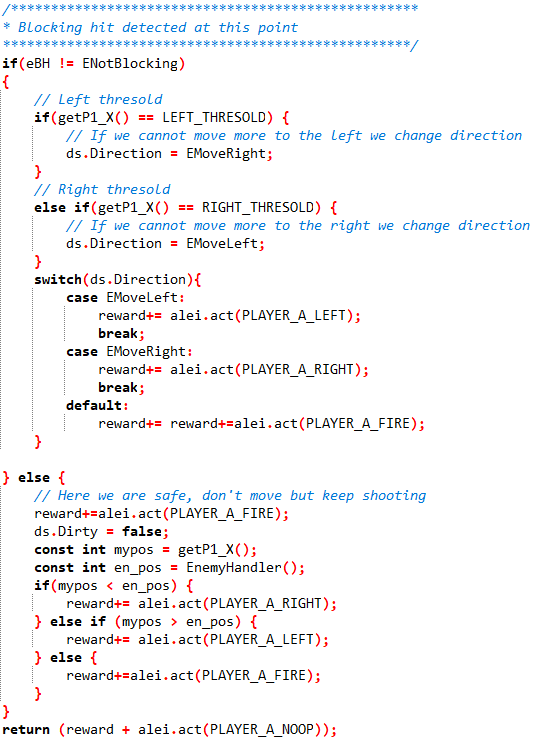
\includegraphics[width=0.79\textwidth]{Figures/damovement}
	\caption{Aplicando movimiento a la nave}
	\label{fig:damovement}
\end{figure}

La parte que extiende a la figura \ref{fig:demonattackp1algo}, es la figura \ref{fig:damovement}. En ésta figura podemos observar la parte del algoritmo que finalmente aplica movimiento a la nave. En este punto ya hemos solucionado la colisión y solo nos queda movernos en la dirección conveniente.

Esta parte del código se divide en dos dependiendo respectivamente si hemos encontrado una colisión o no. En la primera parte ya tenemos en el \textbf{DirtyState} apuntado la dirección en la cual movernos, sin embargo si nos encontramos en los bordes de la pantalla, no nos podremos mover la la dirección del borde, es por esto por lo que cambiamos de dirección cuando llegamos a un borde. Si no estamos en ningún borde, simplemente aplicamos la dirección anotada por \textbf{ds.Direction}.

\begin{figure}[h]
	\centering
	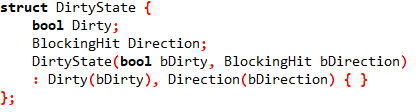
\includegraphics[width=0.79\textwidth]{Figures/structdirtystateda}
	\caption{Struct Dirty State}
	\label{fig:structdirtystateda}
\end{figure}

En la segunda parte, podemos considerar que el jugador uno está a salvo de posibles ataques enemigos, esto viene determinado, como ya hemos comentado anteriormente, por el resultado de isBlockingHit. Por lo tanto, lo que haremos en este modo es disparar siempre que podamos a la vez que intentar traquear a los enemigos en RAM para dispararles dentro de su colisión. \textbf{EnemeyHandler} se encargará de devolvernos el enemigo mas relevante en un instante determinado (usualmente el mas cercano al jugador). Esta función no funciona el 100\% de los casos, ya que como hemos comentado anteriormente, la RAM no es específica a casos concretos sino que va cambiando, por lo tanto habrá, veces que el jugador 1 se quede disparando a la nada porque no tiene nada que trackear. Esto se resuelve parcialmente gracias a la aleatoriedad y al movimiento de las entidades enemigas, que acabaremos matando si se acercan a nuestro láser. La solución completa y real sería llevar un seguimiento mas especifico de todas las unidades en RAM, lo cual puede llevarnos a implementar demasiados casos específicos para un escenario mas simple de solucionar mediante un algoritmo genérico (mediante una buena función de fitness) o un neuroevolutivo en su defecto.


%----------------------------------------------------------------------------------------------%
%----------------------------------------------------------------------------------------------%
%----------------------------------------------------------------------------------------------%
%----------------------------------------------------------------------------------------------%
\newpage
\subsection{Redes neuronales}
\label{subsec:nn}


\newpage